%
%
%
\begin{slide}
\pagestyle{headings}
\sf 
\header{Method of least squares fit - a reminder}
%
\Large
\begin{center}
\begin{figure}[h]
\unitlength1cm
\begin{picture}(15.,9.5)
\put(0.,9.){\underline{Example problem: Particle trajectory measurement}}
\put(0.,2.3){\epsfig{file=feynman/l1.ps,width=6.cm}}
\put(7.,5.6){
\begin{minipage}{5cm}
\underline{general:}\\
$n$-measurements $y_i$ \\
with uncertainties $\sigma_i$\\
at fixed $x_i$\\
\underline{Model:} $ y=f(x,a)$
\end{minipage}
}
\put(0.,2){
\begin{minipage}[t]{13cm}
$\Rightarrow$ how to determine $a$?\\
Idea: for the correct $a$ one expects:
$|y_i - f(x_i,a)|\le \sigma_i$,\\
{\em i.e. curve describes data within 
measurement uncertainties}
\end{minipage}
}
\end{picture}
\end{figure}
\end{center}
\end{slide}
%
%
%
%
%
%
\begin{slide}
\pagestyle{headings}
\sf 
\header{Method of least squares fit - a reminder}
%
\Large
\begin{center}
\begin{figure}[h]
\unitlength1cm
\begin{picture}(15.,9.5)
%
\put(0.,8.){
$\rightarrow$ 
\mbox{\framebox{
$ \chi^2 = \Sigma_{i=1}^n \frac{ (y_i-f(x_i,a))^2}{\sigma_i^2} $}}
$\leftrightarrow \mbox{Minimum with respect to a}$
%\rightarrow \frac{d\chi^2}{da} = 0
%
}
\put(0.,6.5){
$\Rightarrow$ determine a from $\frac{d\chi^2}{da} = 0$
}
\put(0.,5.){
$\rightarrow$ 
\mbox{\framebox{
$ \frac{d\chi^2}{da} = \Sigma_{i=1}^n \frac{ (y_i-f(x_i,a))}{\sigma_i^2} 
\cdot \frac{df(x_i,a)}{da} = 0
$}}
}
\put(0.,3.5){
\begin{minipage}[t]{13cm}
In general not analytically solvable.\\
$\Rightarrow$ use iterative (numerical) methods
(MINUIT, Mathematica) 
\end{minipage}
}
\end{picture}
\end{figure}
\end{center}
\end{slide}


\begin{slide}
\pagestyle{headings}
\sf 
\header{Method of least squares fit - a reminder}
%
\Large
\begin{center}
\begin{figure}[h]
\unitlength1cm
\begin{picture}(15.,9.5)
%
\put(0.,9.){
\begin{minipage}[t]{8cm}
\underline{Most general case}\\
\begin{itemize}
\item  
$y_i,y_j$ correlated measurements with covariance $V_{ij}$
\item 
$m$ fitparameters $\vec{a}$
\end{itemize}
%\vspace*{1cm}
%
\[
\rightarrow
 \begin{array}{|lll|}
\hline
 \chi^2 &  = & \Sigma_{i,j=1}^n 
(y_i - f(x_i,\vec{a}))  V_{ij}^{-1} (y_j - f(x_j,\vec{a}))\\[2mm]
 & = & (\vec{y} - \vec{f}(\vec{a}))^t V^{-1} (\vec{y} - \vec{f}(\vec{a}))\\
\hline
\end{array}
\]
%
\end{minipage} 
%
}
\end{picture}
\end{figure}
\end{center}
\end{slide}




\begin{slide}
\pagestyle{headings}
\sf 
\header{Linear least square fits}
%
\Large
\begin{center}
\begin{figure}[h]
\unitlength1cm
\begin{picture}(15.,9.5)
\put(0.,8.){
\begin{minipage}[t]{15cm}
\Large
$\vec{y}\;$ vector of $n$ measurements
$\left( \begin{array}{l}
y_1(x_1)\\
. \\
y_n(x_n)\\
\end{array}
\right)
\;$
with cov-matrix $ V$\\
\vspace{5mm}

$ \vec{a}\;$ vector of m fitparameters 
$\left( \begin{array}{l}
a_1\\
. \\
a_m\\
\end{array}
\right)
$

%\vspace{2mm}
Model $\vec{y}: \;\; =   A \,\vec{a}$
%
\hspace{1cm}
\underline{Example:} $y=ax$; $\vec{a} = (a)$, 
$ 
A =
\left(
\begin{array}{l}
  x_1  \\
  . .  \\
  x_n  \\
 \end{array}
\right)
$
%\begin{center}
% 

%Master $\chi^2$:
$
\begin{array}{||l||}
\hline
\hline
\chi^2 = \left(\vec{y} - A \, \vec{a}\right)^t V^{-1}
            \left(\vec{y} - A \, \vec{a}\right)
%\quad
\\
\hline
\hline
\end{array}
$

\vspace{1mm}
$\rightarrow$ to be minimised w.r.t $\vec{a}$
%\end{center}
%
\end{minipage}
}
\end{picture}
\end{figure}
\end{center}
\end{slide}

%\begin{slide}
%\pagestyle{headings}
%\sf 
%\header{Examples for linear least square fits}
%%
%\Large
%\begin{itemize}
%\item
%Straight line fit $y_i =a x_i$, $\vec{a}=a$
%\[
%A =
%\left(
%\begin{array}{l}
%  x_1  \\
%  . .  \\
%  x_n  \\
% \end{array}
%\right)
%\]
%\end{itemize}
%\item 
%
%Watch out: linear in $\vec{a}$, 
%{\em but not necessarily in $x$}.\\
%Example fct =  $a e^{-x}$, i.e. model for $y_i$: =   $e^{-x_i}\, a$
%\vspace*{-2mm}
%\end{itemize}
%\end{slide}




\begin{slide}
\pagestyle{headings}
\sf 
\header{Examples for linear least square fits}
\begin{center}
{\em \normalsize Linear means that
$y$ depends linearly on the fitparameters $a_i$.}
\begin{figure}[h]
\unitlength1cm
\begin{picture}(15.,9.5)
%
    \put(1.,-.5){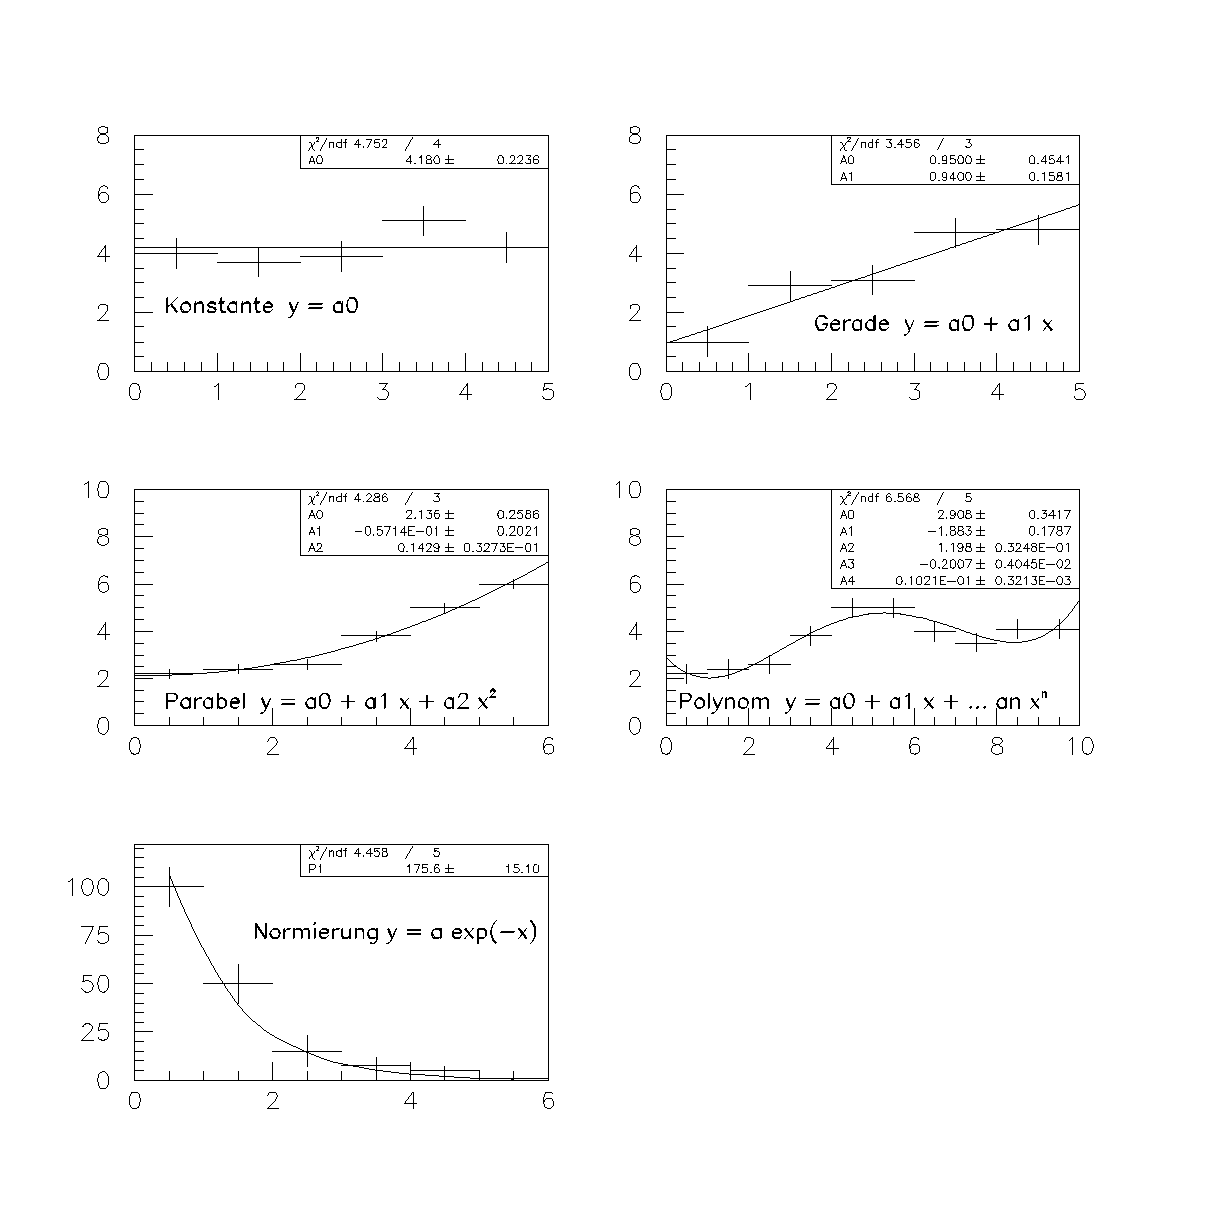
\epsfig{file=eps/linfits.eps,width=11.cm}}
\put(6.,1.){$\leftarrow$ 
\begin{minipage}[t]{5cm}
\em Watch out: function can be highly non-linear in $x$
\end{minipage}
}
\end{picture}
\end{figure}
\end{center}
\end{slide}
%
%
%




